% initial, inherit általános értékekről írni kellene valamit, valahol!

\subsection{Előnyök}

%2
\begin{frame}
  CSS: Cascading Style Sheets
  \begin{itemize}
    \item $\approx$ lépcsőzetes/sorba kapcsolt stíluslapok
    \item \emph{formázás, megjelenés} leírásának elválasztása a \emph{tartalomtól} (HTML), előnyei:
    \begin{itemize}
      \item külön fájlban tárolható, ami több weboldalhoz is használható, így csökken az összesített kódméret, 
      \item egységessé válik ezen oldalak megjelenése,
      \item egymástól függetlenül, egyidejűleg lehet szerkeszteni a formát és a tartalmat,
      \item gyorsabban módosítható a megjelenés, mert csak egy helyen kell változtatni,
      \item hatékonyabbá válik a gyorstárazás,
    \end{itemize}
    \item különféle médiára eltérő formázás lehetséges (pl. képernyő, nyomtatás)
    \item \hiv{\href{http://www.csszengarden.com/}{a CSS ereje}}
    \item \hiv{\href{https://www.w3.org/Style/CSS/learning.en.html}{hivatalos W3C oldal}}
  \end{itemize}
\end{frame}

\subsection{Formázás HTML elemekkel és CSS-sel}

%3
\begin{frame}
  \small
  \begin{alertblock}{Elavult módszer (\textattachfile{htmlFormazas.html}{htmlFormazas.html})}
    \lstinputlisting[style=HTML,numbers=left]{htmlFormazas.html}
  \end{alertblock}
\end{frame}

%4
\begin{frame}
  \scriptsize
  \begin{exampleblock}{Formázás CSS-sel (\textattachfile{cssFormazas.html}{cssFormazas.html})}
    \lstinputlisting[style=HTML,linerange={3-10},numbers=left,firstnumber=3]{cssFormazas.html}
  \end{exampleblock}
  \begin{exampleblock}{Formázás CSS-sel (\textattachfile{cssFormazas.css}{cssFormazas.css})}
    \lstinputlisting[style=HTML,numbers=left]{cssFormazas.css}
  \end{exampleblock}
\end{frame}

\subsection{Szintaktika}

%5
\begin{frame}[fragile]
  \begin{columns}[c]
    \column{0.5\textwidth}
      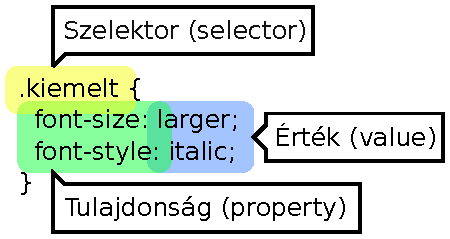
\includegraphics[scale=0.75]{szintakszis.pdf}\\
      \begin{block}{Deklaráció sablonja}
      \vspace{-0.5cm}
\begin{verbatim}
szelektor {
  tulajdonság1: érték(ek);
  tulajdonság2: érték(ek);
  ...
  tulajdonságN: érték(ek);
}
\end{verbatim}
      \vspace{-0.4cm}
      \end{block}
    \column{0.5\textwidth}
      \begin{description}[m]
        \item[Szelektor] \hfill \\ Mit akarunk formázni?
        \item[Tulajdonság] \hfill \\ Milyen tulajdonságán változtassunk?
        \item[Érték] \hfill \\ Milyen legyen az új állapot?
      \end{description}
  \end{columns}
  
\end{frame}

%6
\begin{frame}
  Megjegyzések a CSS-ben:
  \begin{itemize}
    \item \texttt{/* megjegyzes */}
    \item végleges kódból célszerű elhagyni
    \item Lehet több soros is
  \end{itemize} 
  \hiv{\href{https://jigsaw.w3.org/css-validator/}{CSS ellenőrző}}
\end{frame}

\subsection{Egyszerű szelektorok}

%7
\begin{frame}
  \begin{description}[m]
    \item[HTML elem neve] \hfill \\ \texttt{p \{ font-style: italic; \}}
    \item[Egyedi azonosító (\texttt{id} attribútum) alapján] \hfill \\ 
      \texttt{\#lablec \{ font-size: 10pt; \}}\\
      Az \texttt{id} nem kezdődhet számjegy karakterrel!
    \item[Univerzális szelektor, mindenre illeszkedik] \hfill \\ \texttt{* \{ font-size: smaller; \}}
  \end{description}
\end{frame}

%8
\begin{frame}
  \begin{description}[m]
    \item[Osztály (\texttt{class} attribútum alapján)] \hfill \\ 
      \texttt{*.kisbetus \{ font-size: small; \} /* bármilyen HTML elemhez */} \\
      \texttt{.kisbetus \{ font-size: small; \} /* bármilyen HTML elemhez, rövid alak */}\\
      \texttt{p.voros \{ color: red; \} /* csak adott (pl. <p>) HTML elemhez */}\\
      A \texttt{class} értéke nem kezdődhet számjeggyel, de lehet egyszerre több, szóközzel elválasztott értéke: \\
      \texttt{<p class="kisbetus voros">Apróbetűs piros bekezdés</p>}
    \item[Elemek csoportosítása] \hfill \\ \texttt{h1, h2, h3 \{ font-family: Arial; \}}
  \end{description}
\end{frame}

%9
\begin{frame}
  \begin{exampleblock}{\textattachfile{egyszeruSzelektor1.html}{egyszeruSzelektor1.html}}
    \scriptsize
    \lstinputlisting[style=HTML,linerange={3-13},numbers=left,firstnumber=3]{egyszeruSzelektor1.html}
  \end{exampleblock}
\end{frame}

%10
\begin{frame}
  \begin{exampleblock}{\textattachfile{egyszeruSzelektor1.html}{egyszeruSzelektor1.html}}
    \scriptsize
    \lstinputlisting[style=HTML,linerange={14-15},numbers=left,firstnumber=14]{egyszeruSzelektor1.html}
  \end{exampleblock}
\end{frame}

%11
\begin{frame}
  \begin{exampleblock}{\textattachfile{egyszeruSzelektor1.css}{egyszeruSzelektor1.css}}
    \scriptsize
    \lstinputlisting[style=HTML,numbers=left]{egyszeruSzelektor1.css}
  \end{exampleblock}
  \begin{center}
    
\includegraphics[width=.9\textwidth]{egyszeruSzelektor1.png}
  \end{center}
\end{frame}

\subsection{Stílusok forrása}

%12
\begin{frame}
  Háromféle helyen lehet stílusokat megadni:
  \begin{enumerate}
    \item Külső fájlban (\texttt{css} kiterjesztés, \texttt{<link>} elem)
    \item A \texttt{<head>} elembe ágyazott \texttt{<style>} elemben. Csak akkor ajánlott, ha egyetlen HTML fájlt kívánunk formázni ezekkel a stílusokkal.
    \item Soron belül: a HTML elemek \texttt{style} attribútumának értékeként. Ismét \kiemel{keveredik a tartalom a stílussal}, ezért általában \kiemel{nem ajánlott} a használata!
  \end{enumerate}
\end{frame}

%13
\begin{frame}
  \begin{exampleblock}{\textattachfile{egyszeruSzelektor2.html}{egyszeruSzelektor2.html}}
    \footnotesize
    \lstinputlisting[style=HTML,linerange={3-12},numbers=left,firstnumber=3]{egyszeruSzelektor2.html}
    \lstinputlisting[style=HTML,linerange={16-16},numbers=left,firstnumber=16]{egyszeruSzelektor2.html}
  \end{exampleblock}
\end{frame}

\subsection{Ütközések feloldása}

%14
\begin{frame}
  Ha több előírás is vonatkozik ugyanannak az objektumnak a formázására, elsőként a forrás prioritása dönt (csökkenő sorrendben):
  \begin{enumerate}
    \item soron belüli formázások
    \item külső és belső (\texttt{<link>}, \texttt{<style>} elemek) formázások
    \item böngésző alapértelmezése
  \end{enumerate}
  Azonos prioritás (pl. két külső stíluslap) esetén a később betöltött szabály felülírja a korábbit.
\end{frame}

%15
\begin{frame}
  \begin{exampleblock}{\textattachfile{utkozes1.html}{utkozes1.html}}
    \scriptsize
    \lstinputlisting[style=HTML,linerange={6-13},numbers=left,firstnumber=6]{utkozes1.html}
  \end{exampleblock}
  \begin{columns}[T]
    \column{0.6\textwidth}
      \begin{exampleblock}{\textattachfile{utkozes1.css}{utkozes1.css}}
        \scriptsize
        \lstinputlisting[style=HTML,numbers=left,firstnumber=1]{utkozes1.css}
      \end{exampleblock}
    \column{0.3\textwidth}
      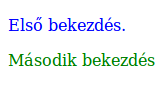
\includegraphics[width=.66\textwidth]{utkozes1.png}
  \end{columns} 
\end{frame}

%16
\begin{frame}
  \begin{exampleblock}{\textattachfile{utkozes2.html}{utkozes2.html}}
    \scriptsize
    \lstinputlisting[style=HTML,linerange={6-13},numbers=left,firstnumber=6]{utkozes2.html}
  \end{exampleblock}
  \begin{columns}[T]
    \column{0.6\textwidth}
      \begin{exampleblock}{\textattachfile{utkozes1.css}{utkozes1.css}}
        \scriptsize
        \lstinputlisting[style=HTML,numbers=left,firstnumber=1]{utkozes1.css}
      \end{exampleblock}
    \column{0.3\textwidth}
      
\includegraphics[width=.66\textwidth]{utkozes2.png}
  \end{columns} 
\end{frame}

\subsection{Színek}

%17
\begin{frame}
  Számtalan dolognak beállítható a színe CSS tulajdonságokkal, pl.:
  \begin{description}[m]
    \item[\texttt{color}] \hfill \\ Szöveg írásszíne
    \item[\texttt{background-color}] \hfill \\ Háttérszín
  \end{description}
  Szín, mint a tulajdonság értéke megadható:
  \begin{description}[m]
    \item[kulcsszavakkal] \hfill \\ Pl. \texttt{red} (vörös), 
    \texttt{green} (zöld), \texttt{blue} (kék), \texttt{white} (fehér), 
    \texttt{black} (fekete), \dots \\
    \hiv{\href{https://www.w3.org/TR/css-color-3/\#svg-color}%
    {140 szabványos színkód}}
    \item[Hexadecimálisan, RGB összetevőkkel] \hfill \\ Pl. 
    narancsszín: \texttt{\#ff7f00}, ahol \texttt{\#} jelzi a 16-os 
    számrendszerbeli alakot, \texttt{ff} a vörös (\kiemel{R}ed), 
    \texttt{7f} a zöld (\kiemel{G}reen) és \texttt{00} a kék 
    (\kiemel{B}lue) összetevő intenzitása 8 biten előjel nélkül, 
    fixpontosan. Additív színkeverés.
  \end{description}
\end{frame}

%18
\begin{frame}
  \begin{description}[m]
    \item[\texttt{rgb()} függvénnyel] \hfill \\ \texttt{rgb(red, 
    green, blue)}, ahol mindhárom összetevő lehet 0-255 közötti 
    decimális egész, vagy 0-100\%. Pl. \texttt{rgb(255,0,0)} vagy 
    \texttt{rgb(100\%, 0\%, 0\%)} vörös színt eredményez.
    \item[\texttt{rgba()} függvénnyel] \hfill \\ \texttt{rgb(red, 
    green, blue, alpha)}, ahol a színösszetevőket egy 
    átlátszóság érték követi ([0, 1]).
  \end{description}
  \vfill
  \begin{center}
    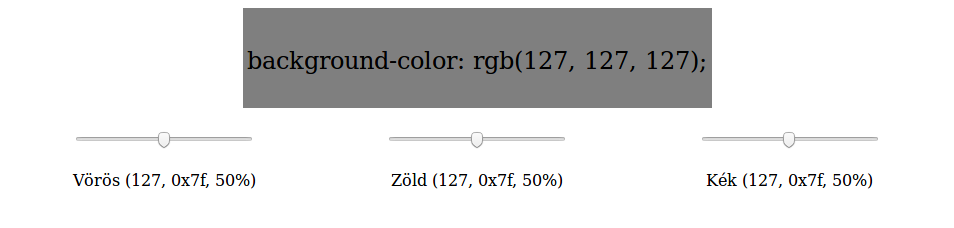
\includegraphics[scale=0.2]{szinek1.png}\\
    \textattachfile{szinek1.html}{szinek1.html}
  \end{center}
\end{frame}

%19
\begin{frame}
  \begin{description}[m]
    \item[\texttt{hsl()} függvénnyel] \hfill \\ \texttt{hsl(hue, 
    saturation, lightness)}, ahol \texttt{hue} az árnyalat, [0, 360] 
    fok közötti elfordulás a színkeréken. Pl. 0$^{\circ}$ a 
    vöröshöz, 120$^{\circ}$ a zöldhöz, 240$^{\circ}$ a kékhez 
    tartozik. \texttt{saturation} a telítettség, százalékban. A 0\% 
    a színinformáció hiányát (szürkeség) jelzi, 100\% a teljes 
    színezettséget. \texttt{lightness} a fényesség, szintén 
    százalékban. A 0\% mindig fekete, a 100\% mindig fehér színt ad.
    \item[\texttt{hsla()} függvénnyel] \hfill \\ A fentiek 
    kiegészülnek átlátszósággal.
  \end{description}
  \vfill
  \begin{center}
    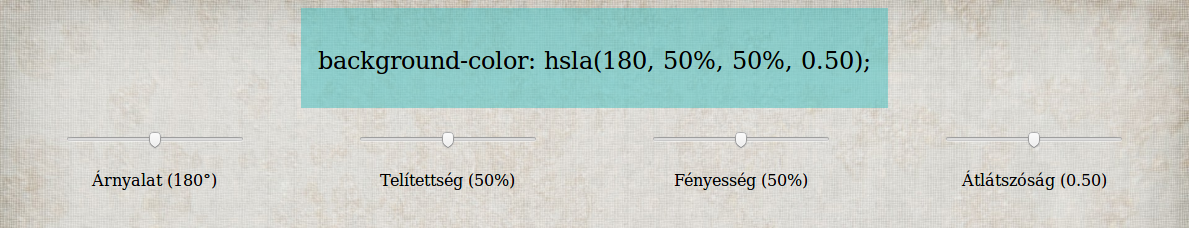
\includegraphics[scale=0.2]{szinek2.png}\\
    \textattachfile{szinek2.html}{szinek2.html}
  \end{center}
\end{frame}

%20
\begin{frame}
  \begin{columns}[c]
    \column{0.5\textwidth}
      Induljon ki a \textattachfile{szinezes.html}{szinezes.html} 
      fájlból! Kapcsolja ezt össze egy külső stíluslappal, majd 
      érje el, hogy a jobb oldali ábrának megfelelő színekben 
      pompázzon! Próbáljon minél több féle szín megadási 
      módszert alkalmazni! Törekedjen a lehető legtömörebb CSS 
      szabályok megalkotására!
    \column{0.5\textwidth}
      \begin{exampleblock}{\textattachfile{szinezes-mo.html}{szinezes-mo.html}, 
        \textattachfile{szinezes-mo.css}{szinezes-mo.css}}
        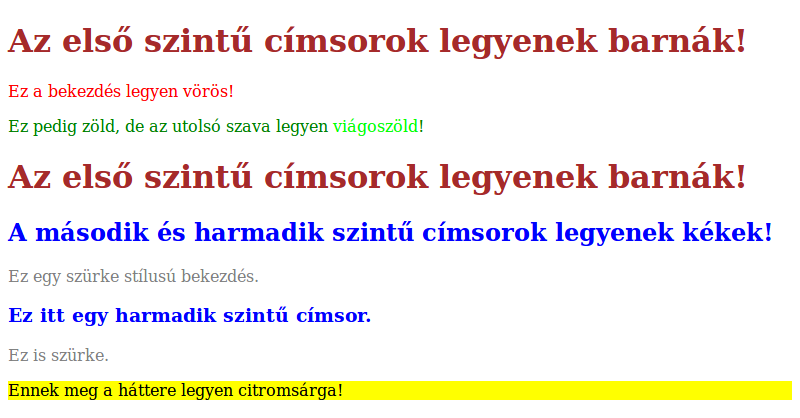
\includegraphics[width=\textwidth]{szinezes-mo.png}
      \end{exampleblock}
  \end{columns} 
\end{frame}

\subsection{Háttér}

%21
\begin{frame}
  HTML elemek hátterével kapcsolatos tulajdonságok:
  \begin{description}[m]
    \item[\texttt{background-color}] \hfill \\ A háttér színe. 
    Alapértelmezetten \texttt{transparent}, azaz átlátszó.
    \item[\texttt{background-image}] \hfill \\ Háttérkép, amivel 
    alapértelmezés szerint kicsempézi az elem teljes területét 
    (margókat nem). 
    Alapértéke \texttt{none}, nincs háttérkép. Az \texttt{url()} 
    függvény paramétereként adható meg a képfájl, pl. \\
    \texttt{background-color: url("hatter.png");} \\Megadhatók 
    \hiv{\href{https://cssgradient.io/}{színátmenetek}} is.\\
    A szöveg maradjon \kiemel{olvasható} a háttéren!
  \end{description}
\end{frame}

%22
\begin{frame}
  \begin{description}[m]
    \item[\texttt{background-repeat}] \hfill \\ Háttérkép 
    csempézési iránya
    \begin{itemize}
      \item \texttt{repeat} mindkét irányban, túlnyúló részek 
      levágásával, alapértelmezés
      \item \texttt{repeat-x} csak vízszintesen
      \item \texttt{repeat-y} csak függőlegesen
      \item \texttt{no-repeat} csak egyszer, alapértelmezetten a bal 
      felső sarokban
      \item \texttt{round} torzítja a képet a vágás elkerülésére
      \item \texttt{space} csak annyiszor ismétel, ami vágás 
      nélkül elfér, közöttük helyet hagy
    \end{itemize}
    Két érték megadásakor az első a vízszintes, második a 
    függőleges irányra vonatkozik.
  \end{description}
\end{frame}

%23
\begin{frame}
  \begin{center}
    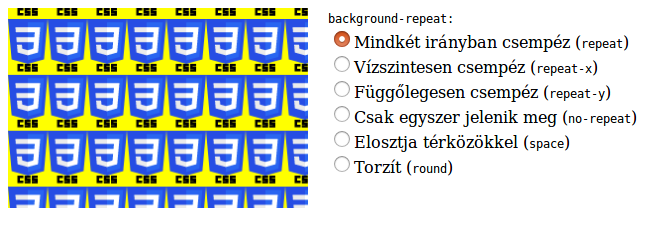
\includegraphics[width=.75\textwidth]{hatter.png}\\
    \textattachfile{hatter.html}{hatter.html}
  \end{center}
\end{frame}

%24
\begin{frame}
  \begin{description}[m]
    \item[\texttt{background-position}] \hfill \\ Igazítás, a 
      \emph{vízszintes} és a \emph{függőleges} pozíciót várja. Ha egyet 
      kap, a másik \texttt{center} lesz.
      \begin{itemize}
        \item Függőlegesen: \texttt{left}, \texttt{center}, 
        \texttt{right}
        \item Vízszintesen: \texttt{top}, \texttt{center}, 
        \texttt{bottom}
        \item Mindkettőnél lehet százelékot, vagy egyéb CSS 
        mértékegységet (pl. képpont) használni. 
      \end{itemize}
  \end{description}
\end{frame}

%25
\begin{frame}
  \begin{exampleblock}{\textattachfile{pozicio1.html}{pozicio1.html}}
    \fontsize{7}{8} \selectfont
    \lstinputlisting[style=HTML,linerange={7-11},numbers=left,firstnumber=7]{pozicio1.html}
    \lstinputlisting[style=HTML,linerange={15-16},numbers=left,firstnumber=15]{pozicio1.html}
    \lstinputlisting[style=HTML,linerange={24-25},numbers=left,firstnumber=24]{pozicio1.html}
    \lstinputlisting[style=HTML,linerange={37-38},numbers=left,firstnumber=37]{pozicio1.html}
    \lstinputlisting[style=HTML,linerange={53-54},numbers=left,firstnumber=53]{pozicio1.html}
  \end{exampleblock}
\end{frame}

%26
\begin{frame}
  \begin{description}[m]
    \item[\texttt{background-attachment}] \hfill \\
      \begin{itemize}
        \item \texttt{scroll} a háttér együtt gördül az oldallal, 
        alapértelmezés
        \item \texttt{fixed} rögzített háttér
        \item \texttt{local} az elem tartalmával együtt gördül a háttér
      \end{itemize}
      \vfill
      A logo mindig a jobb alsó sarokban: 
      \textattachfile{rogzites1.html}{rogzites1.html}\\
      Két bekezdés között kilátszik a háttérben rögzített logo: 
      \textattachfile{rogzites2.html}{rogzites2.html}
  \end{description}
\end{frame}

%27
\begin{frame}
  \begin{description}[m]
    \item[\texttt{background}] \hfill \\ Rövidítés: egy összetett 
    tulajdonsággal sok egyszerű tulajdonság értéke állítható 
    be. \kiemel{Értékek sorrendje rögzített, de tetszőleges 
    számú érték elhagyható!}\\
    \texttt{background: \emph{background-color background-image 
    background-repeat}\\
    \qquad\emph{background-attachment background-position}}
  \end{description}
  \begin{columns}[T]
    \column{0.5\textwidth}
      \begin{exampleblock}{\textattachfile{pozicio1.html}{pozicio1.html}}
        \fontsize{7}{8} \selectfont
        \lstinputlisting[xleftmargin=-1cm,style=HTML,linerange={7-11}]{pozicio1.html}
      \end{exampleblock}
    \column{0.5\textwidth}
      \begin{exampleblock}{\textattachfile{pozicio2.html}{pozicio2.html}}
        \fontsize{7}{8} \selectfont
        \lstinputlisting[xleftmargin=-1cm,style=HTML,linerange={7-10}]{pozicio2.html}
      \end{exampleblock}
  \end{columns} 
\end{frame}

%28
\begin{frame}
  \begin{description}[m]
    \item[\texttt{background-size}] \hfill \\
      \begin{itemize}
        \item \texttt{auto}: Alapértelmezés, eredeti méret.
        \item \emph{szélesség, magasság}: utóbbi elhagyásával 
        \texttt{auto}-t feltételez. Használhatók CSS 
        mértékegységek és százalékok (\kiemel{a szülő elem mérete a 
        100\%}, nem a sajátja!).
        \item \texttt{cover} Addig nyújt és vág, amíg le nem fedi a 
        szülő elem teljes területét.
        \item \texttt{contain} Addig nyújt, amíg egyszer bele nem fér a 
        háttér a szülő elembe.
      \end{itemize}
  \end{description}
  \vfill
  \begin{center}
    
\includegraphics[scale=0.3]{meret.png}\\
    \textattachfile{meret.html}{meret.html}
  \end{center}
\end{frame}

%29
\begin{frame}
  \begin{columns}[c]
    \column{0.5\textwidth}
      \footnotesize
      Induljon ki a \textattachfile{rogzites2.html}{rogzites2.html} 
      fájlból, és alakítsa át a jobb oldali ábrának megfelelően!
      \begin{itemize}
        \item Az írásszín legyen világos szürke!
        \item A teljes oldal háttere legyen kék (RGB-összetevők: 0, 
        145 és 190)!
        \item A \texttt{<div>} elem háttereként állítsa be a 
        \textattachfile{HTML5sticker.png}{HTML5sticker.png} fájl!
        \item Ennek helyzete ne függjön a görgetéstől!
        \item Helyezze el azt a képernyő közepén!
        \item A képet méretezze aránytartó módon úgy, hogy éppen 
        kitöltse a rendelkezésre álló helyet!
        \item Próbálja mindezt a lehető legkevesebb CSS tulajdonság 
        felhasználásával elérni!
      \end{itemize}
    \column{0.5\textwidth}
      \begin{exampleblock}{\textattachfile{rogzites3-mo.html}{rogzites3-mo.html}, \textattachfile{HTML5sticker.png}{HTML5sticker.png}}
        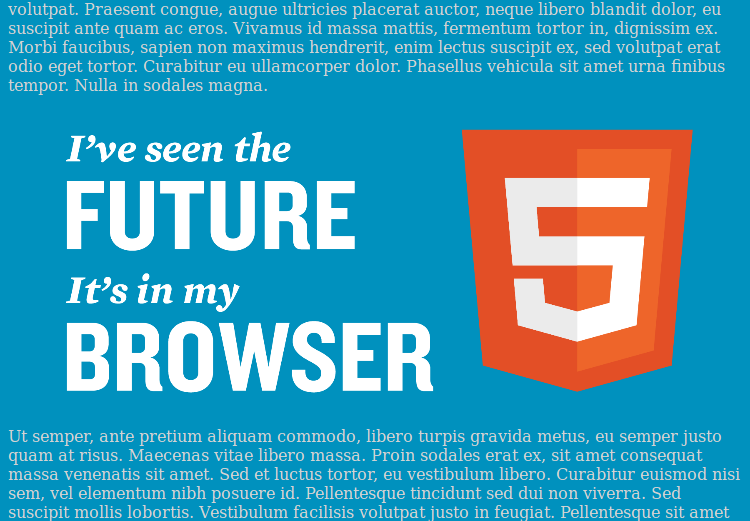
\includegraphics[width=\textwidth]{rogzites3-mo.png}
      \end{exampleblock}
  \end{columns} 
\end{frame}
